%\textbf{Problem statement: } \texit{Write a pass that counts the number of times each instruction is used when a program is executed.} \\
%\textbf{Problem instance:}

\subsection{Pass Algorithm Description}
We want to write a pass which counts the number of times each instruction is used when a program is executed. We cannot do this by a simple static analysis of the program, we need to instrument its bitcode by adding instructions that will count each instruction in the initial program whenever it is used during the execution, while making sure the instructions we added are not counted themselves.

\begin{algorithm}[here]
%\SetKwFunction{count}{count}
%\SetKwFunction{print}{print}
\textbf{count}(Instructions $I_B$)  \Begin {
	\ForEach{$i \in I_B$}{
	 	\If{$M$.containsKey($i$)} {
 			$M$.valueForKey($i$)+=1
	 	}
 		\Else {
 			$M$.insertKeyValuePair($<i$,$1>$)
 		}
	}
}
\textbf{print}() \Begin{
	$t = 0$ \\
	 \ForAll{keyValuePair $\in M$} {
 		print("Found "keyValuePair.value() "counts of: "keyValuePair.key())\\
	 	$t$ += keyValuePair.value()
	 }
	 print("total instructions: "$t$)
}

\caption{Functions inserted in the input program; $I_B$ is the set of instruction for a given basic block}
\end{algorithm}

To achieve this purpose, we insert a counting function and a printing function (both of which can be seen on algorithm 2) in the input programs, as well as calls to that function at the end of each basic block (see figure 1). Given that all instructions in a basic block are executed atomically, a single call to the counting function is sufficient.

\begin{figure}[here]
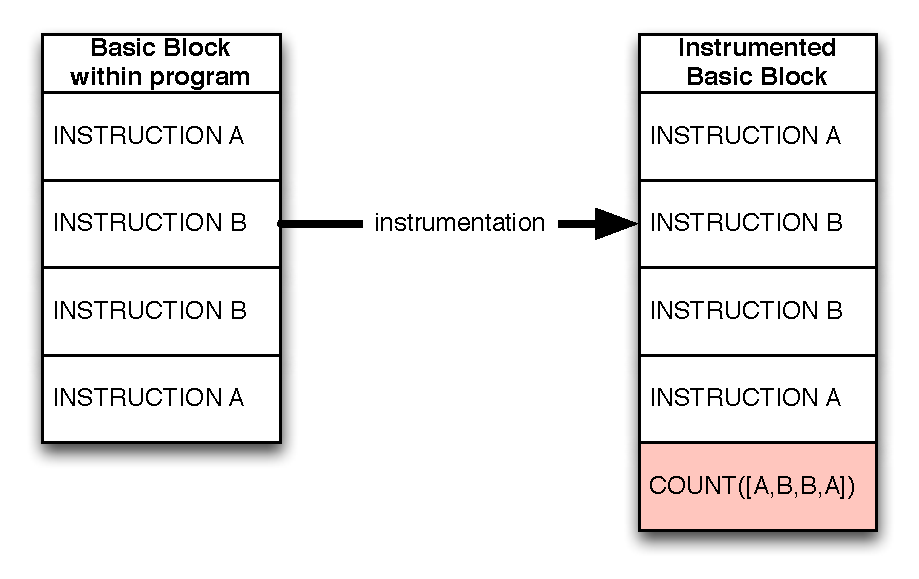
\includegraphics[width=0.4\textwidth]{instructionbitcode}
\caption{bitcode instrumentation}
\end{figure}

\subsection{Physical Implementation Description}

Functions shown on algorithm 2 are written in C++, compiled separately and then linked to the input program later (as described in the instructions), but calls to these functions have to be inserted using the \code{opt} pass.

Again, we used the \code{ModulePass} class and \code{RunOnModule(Module \&M)} method for the implementation. First, we iterate through each basic block (using the \code{Module} and \code{Function} iterators) and collect the instructions for that block using the \code{CI.getOpcodeName()} method provided by the LLVM library for each instruction \code{CI}. We then concatenate all of these instructions into some comma separated string called \code{result}. Finally, we use the following code snippet to call the linked function :

\begin{frame}[fragile]
%\frametitle{Inserting source code}
\lstset{language=C++,
                basicstyle=\ttfamily,
                keywordstyle=\color{blue}\ttfamily,
                stringstyle=\color{red}\ttfamily,
                commentstyle=\color{cool}\ttfamily,
                morecomment=[l][\color{magenta}]{\#}
}
\begin{lstlisting}
// BE points to the end of the BB
builder.SetInsertPoint(BB,BE);
Value* myStr = 
builder.CreateGlobalStringPtr(result);
builder.CreateCall(hookCount,myStr);
\end{lstlisting}
\end{frame}
As can be seen from this snippet, we used an \code{IRBuilder} class to help constructing the call insertion. We did not have to concatenate instructions (we could have used an array of strings), but strings are easier to pass to call instructions using the LLVM library than arrays of strings. Notice that the C++ implementation of the \code{count} function accepts a \code{char*} as input, accordingly.

\subsection{Benchmark Analysis}

In the execution of the gcd example, the main function calls the \code{gcd()} function on input \code{(72,32)}. We can easily predict that the \code{gcd} will be called twice recursively before returning to main, which in turn will return at the end of execution. No other function calls are made. As such we should expect the \code{ret} instruction to be called 4 times, which is precisely the number of times it is called in the benchmark we generated.
